\chapter{Methylamine survey in Orion-KL
\label{chap:Orion-KL}}

\section{Observation data}
%\subsection{Cycle 2}
%\subsection{ALMA Science Verification data}

\section{Analysis}
\subsection{Continuum Subtraction of SV data}


\subsection{Line identification}

1.We drew methylamine emission maps using Common Astronomy Software Applications (CASA) software (McMullin et al.2007). 
We used JPL Molecular Spectroscopy catalog to identify the transition lines. 
8 spectral features exhibit a compact emission at the center of the Hot core . 
We extracted spectrum from this region.

2. We estimated the systemic velocity and the line width of 217.758 GHz line, 
reported by Pagani et al. (2017), which seem contaminated by 
other lines.

3. Using these value, we obtained the integrated 
intensity of 8 transitions described in Table \ref{tab1} by Gaussian fitting.



\section{Results}
\subsection{Transitions}

\begin{table}[htb]
\begin{center}

  \caption{Observed rotational transitions of CH$_3$NH$_2$ in Orion-KL}
  \label{tab1}
{\scriptsize
  \begin{tabular}{|c|c|c|c|l|} \hline
   Fequency [GHz]& S$\mu ^{2}$ [D$^2$] & E$_{\rm{u}}$ [K]& Transition ($J$, $K_{\rm{a}}$, $\Gamma$) & Comments \\ \hline 
    215.670 & 53.92 & 111.48 & 9, 2, $E_{1-1}$ $\rightarrow$ 9, 1, $E_{1+1}$ & Partially blended \\
    245.202 & 37.84 & 168.31 & 12, 1, $B_{2}$ $\rightarrow$ 11, 2, $B_{1}$ &  \\
    217.758 & 129.88 & 182.05 & 12, 2, $B_{2}$ $\rightarrow$ 12, 1, $B_{1}$ & \\
    221.755 & 35.06 & 133.11 & 10, 2, $A_{2}$ $\rightarrow$ 10, 1, $A_{1}$ & \\
    229.908 & 27.37 & 92.71 & 8, 2, $A_{2}$ $\rightarrow$ 8, 1, $A_{1}$ & \\ 
    235.735 & 82.06 & 92.76 & 8, 2, $B_{2}$ $\rightarrow$ 8, 1, $B_{1}$ & \\
    242.262 & 60.23 & 60.86 & 6, 2, $B_{2}$ $\rightarrow$ 6, 1, $B_{1}$ & \\
    244.887 & 49.54 & 48.09 & 5, 2, $B_{1}$ $\rightarrow$ 5, 1, $B_{2}$ & \\ \hline
  \end{tabular}
  }
\end{center}
\end{table}

\subsection{Distribution}

%%%%% 積分強度図挿入 %%%%%
\begin{figure}[htbp] 
\begin{center}
\begin{minipage}{0.98\textwidth} 
\begin{center}
%%%% ここから
\begin{minipage}{0.48\textwidth}
\begin{center}
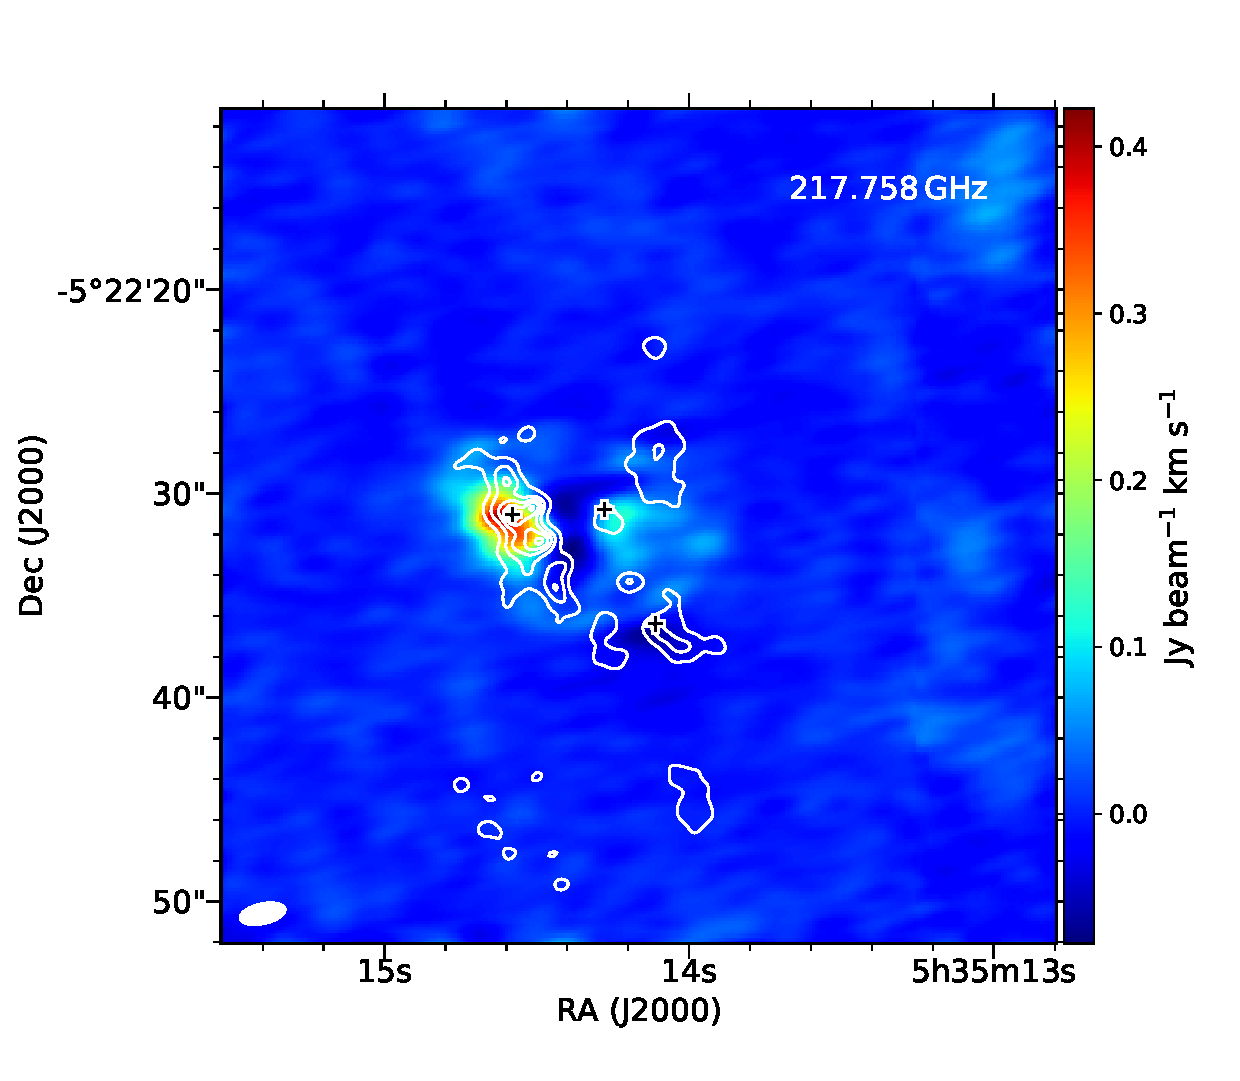
\includegraphics[width=0.98\textwidth]{OrionKL/mom0/217.758mom0_3-7.eps}
%\\(a) 左の図の説明
\end{center}
\end{minipage}
\begin{minipage}{0.48\textwidth}
\begin{center}
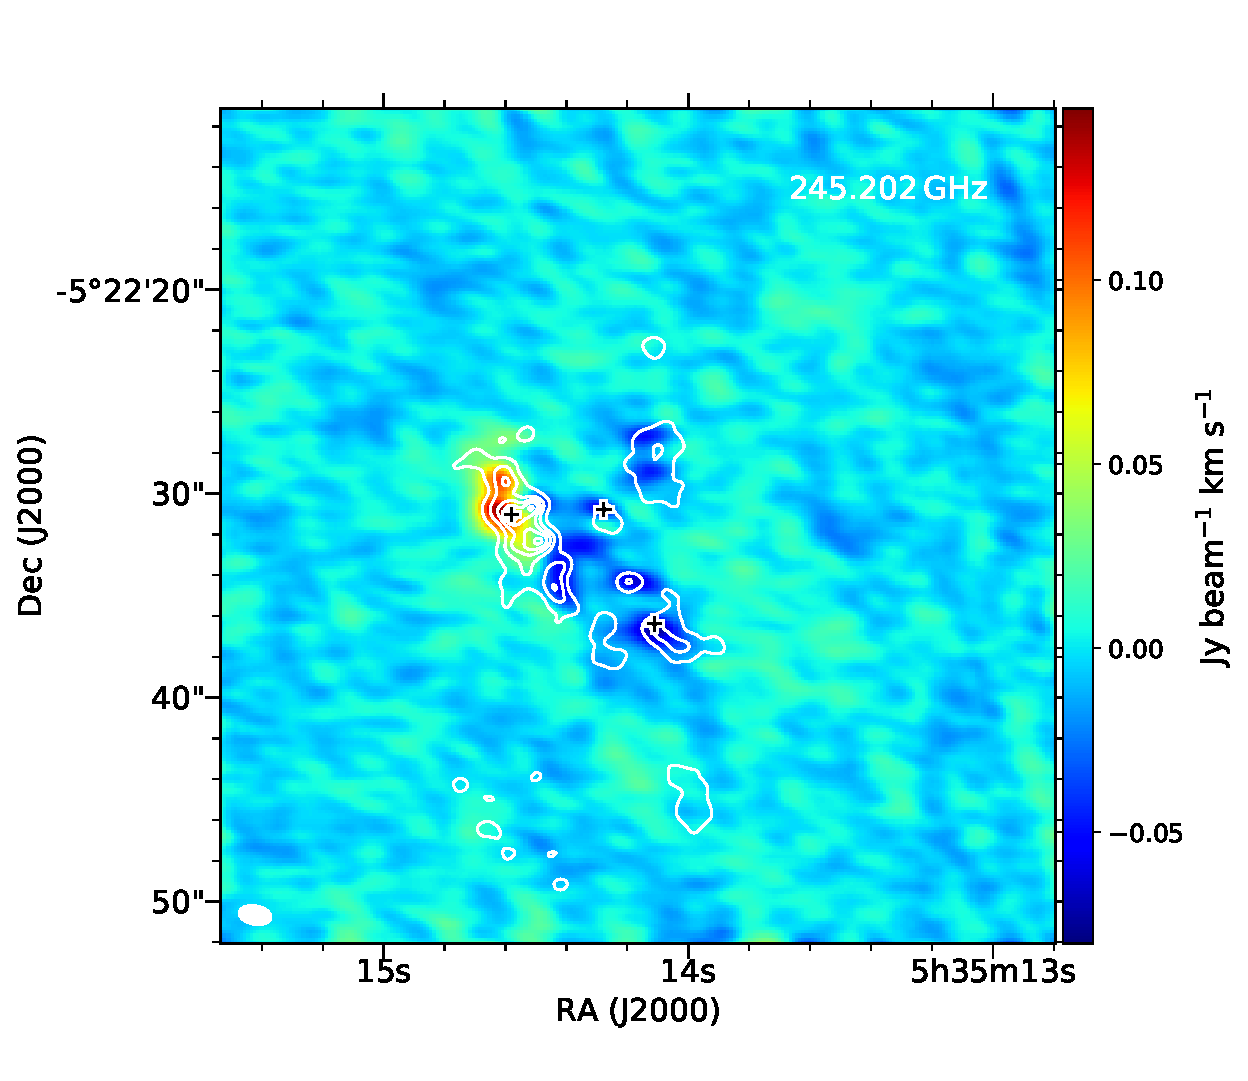
\includegraphics[width=0.98\textwidth]{OrionKL/mom0/245.202mom0_3-7.eps}
%\\(b) 右の図の説明
\end{center}
\end{minipage}
\end{center}
\end{minipage}
%%%% ここまで一組

\begin{minipage}{0.98\textwidth} 
\begin{center}
\begin{minipage}{0.48\textwidth}
\begin{center}
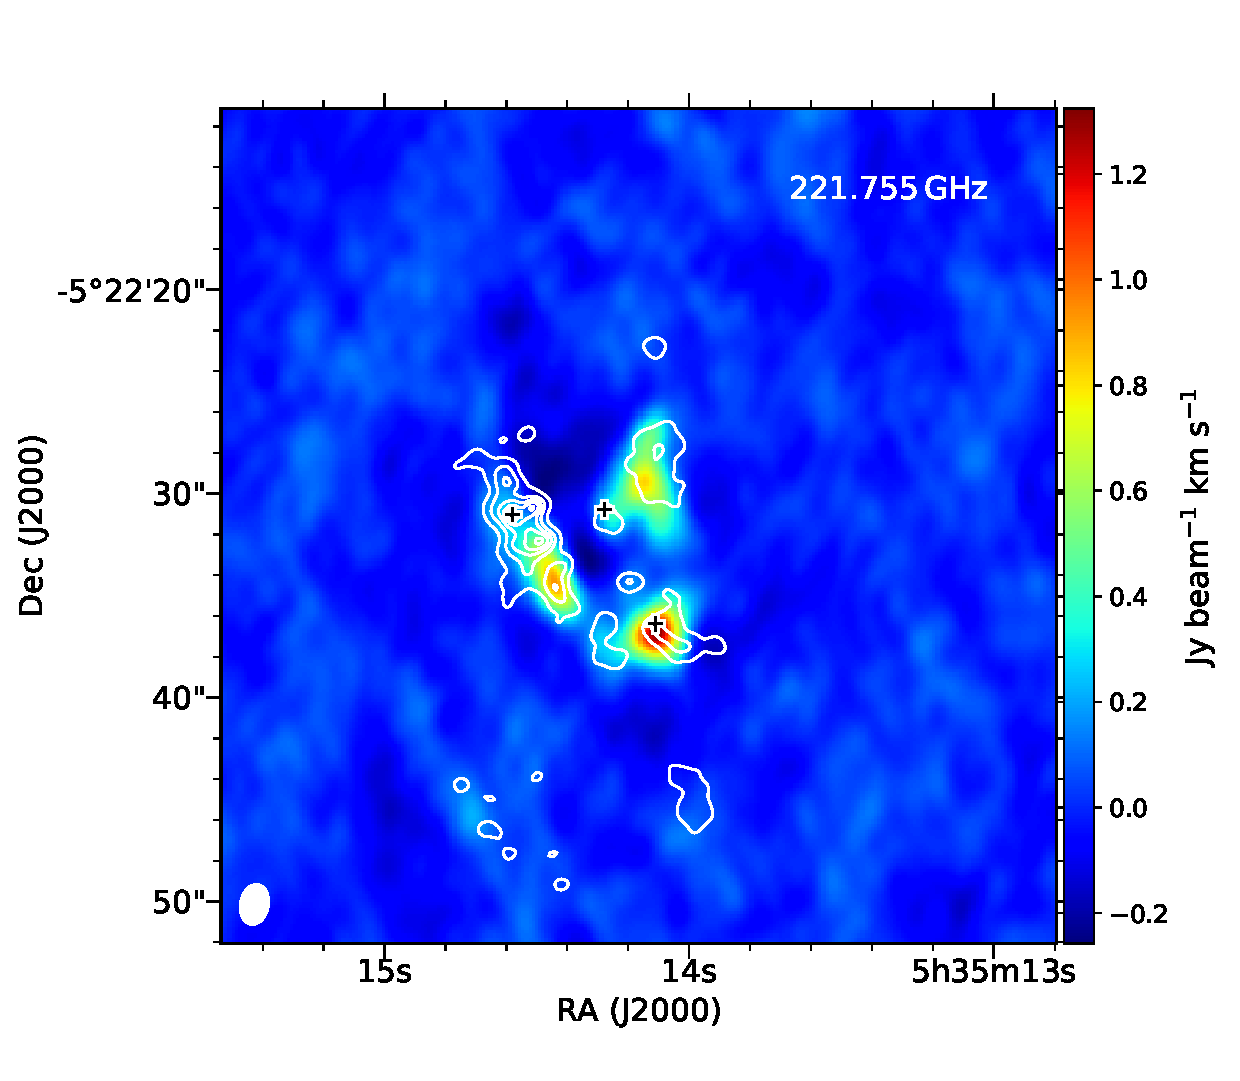
\includegraphics[width=0.98\textwidth]{OrionKL/mom0/221.755SV_mom0_3-7.eps}
%\\(c) 左の図の説明
\end{center}
\end{minipage}
\begin{minipage}{0.48\textwidth}
\begin{center}
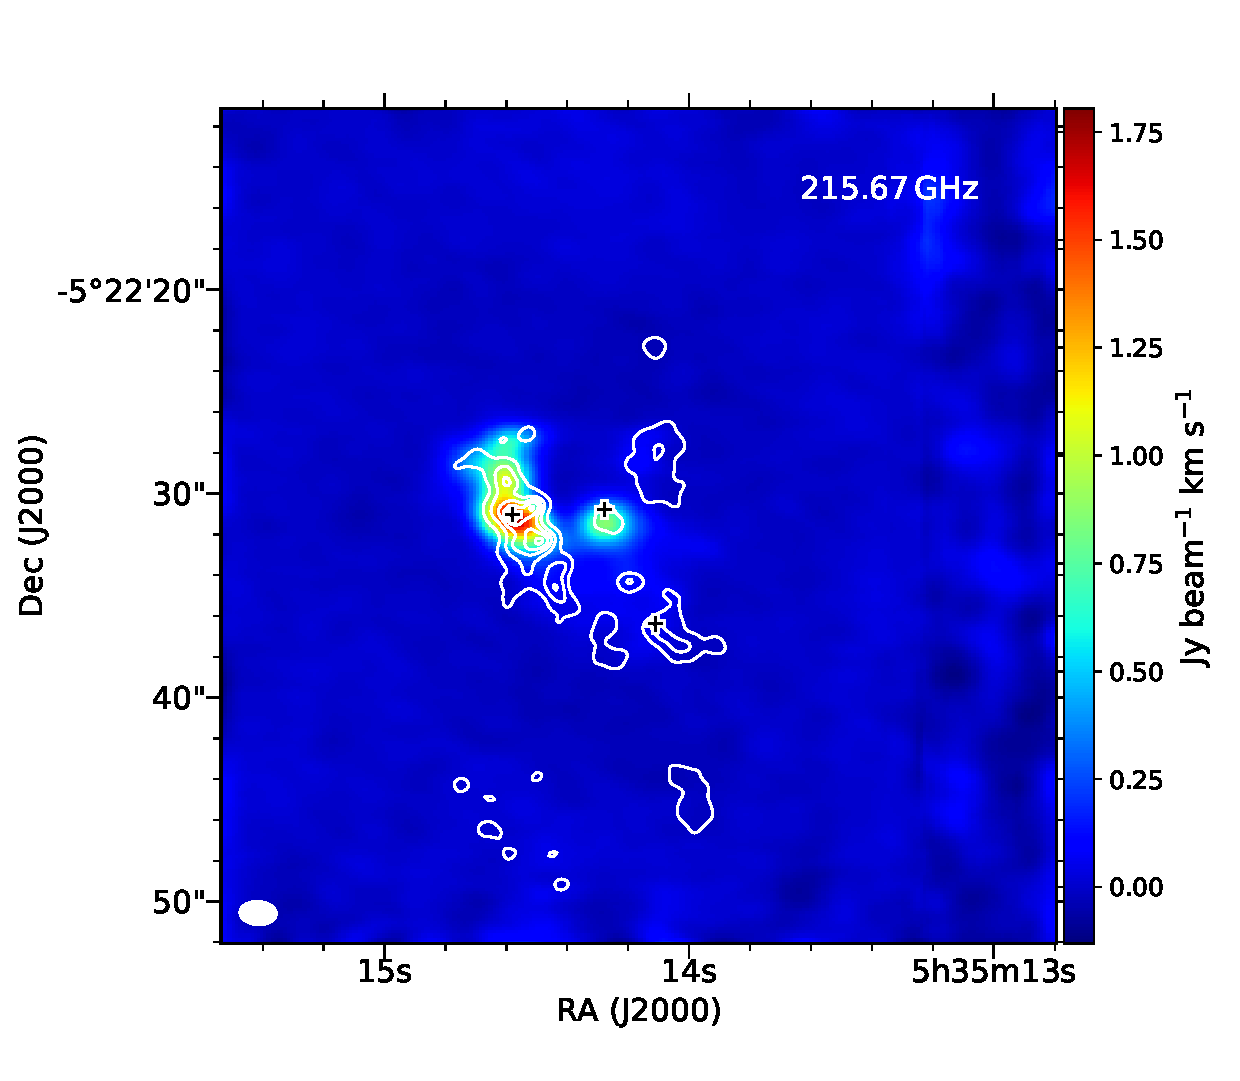
\includegraphics[width=0.98\textwidth]{OrionKL/mom0/215.67mom0_3-7.eps}
%\\(d) 右の図の説明
\end{center}
\end{minipage}
\end{center}
\end{minipage}

\caption{Integrated intensity map}
\end{center}
\end{figure}

\newpage

\begin{figure}[htbp] 
\begin{center}
\begin{minipage}{0.98\textwidth} 
\begin{center}
%%%% ここから
\begin{minipage}{0.48\textwidth}
\begin{center}
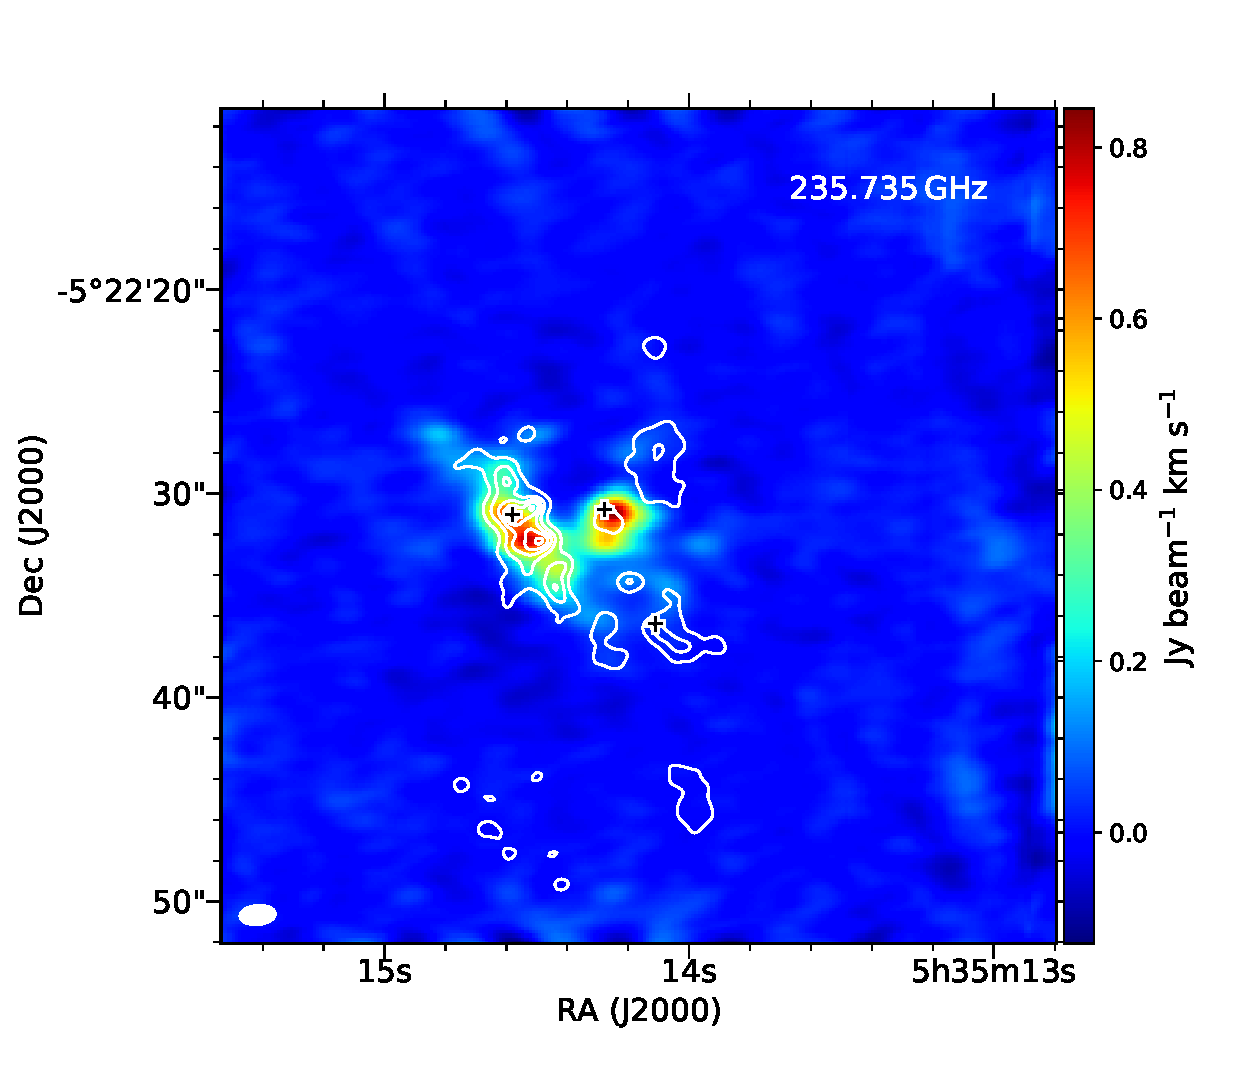
\includegraphics[width=0.98\textwidth]{OrionKL/mom0/235.735mom0_3-7.eps}
%\\(e) 左の図の説明
\end{center}
\end{minipage}
\begin{minipage}{0.48\textwidth}
\begin{center}
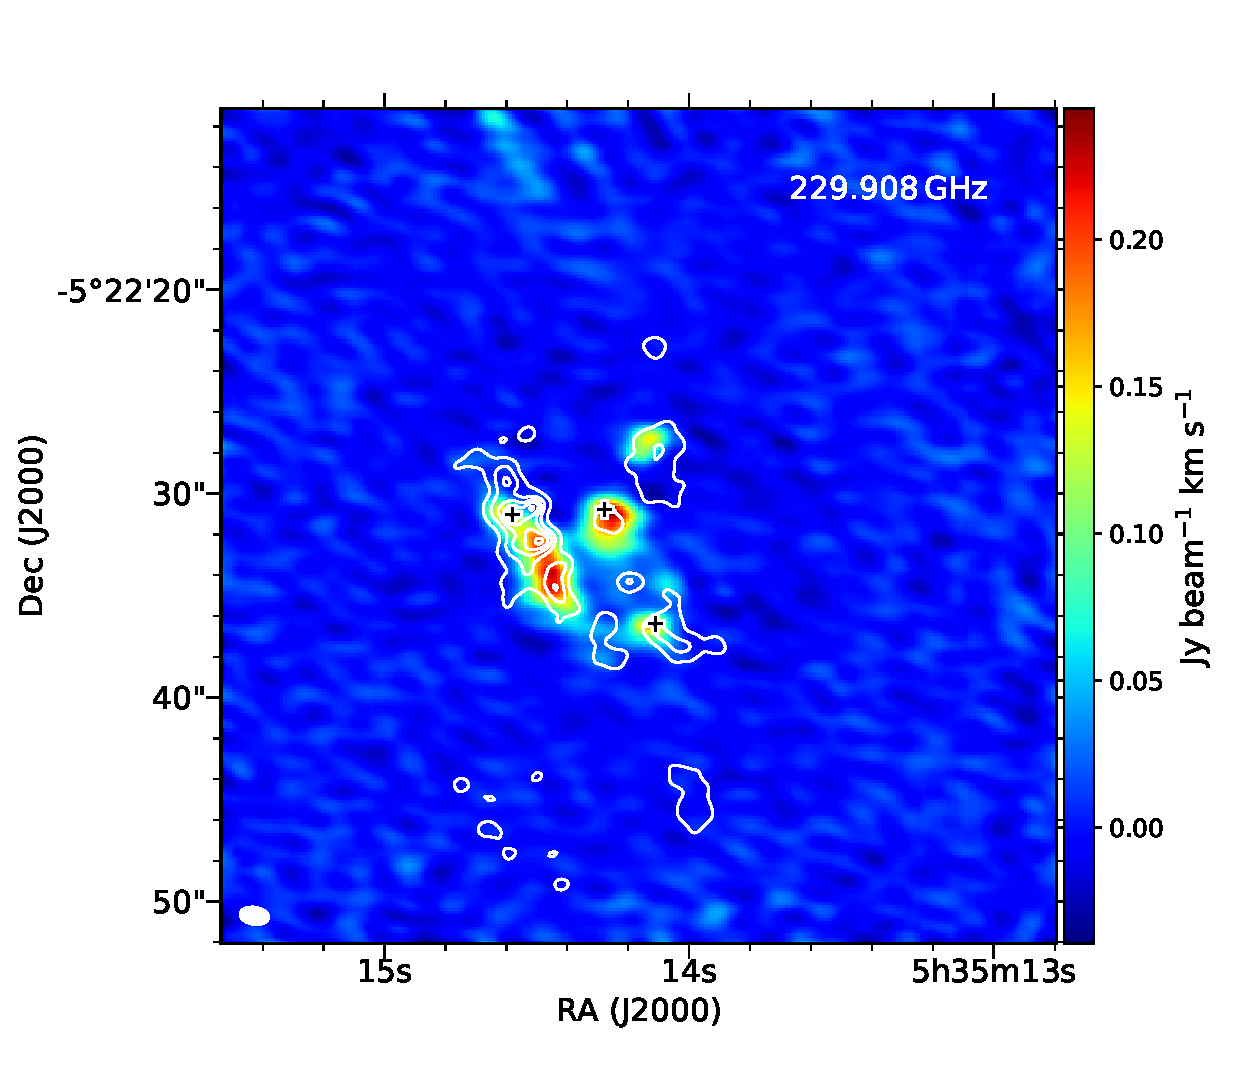
\includegraphics[width=0.98\textwidth]{OrionKL/mom0/229.908mom0_3-7.eps}
%\\(f) 右の図の説明
\end{center}
\end{minipage}
\end{center}
\end{minipage}
%%%% ここまで一組

\begin{minipage}{0.98\textwidth} 
\begin{center}
\begin{minipage}{0.48\textwidth}
\begin{center}
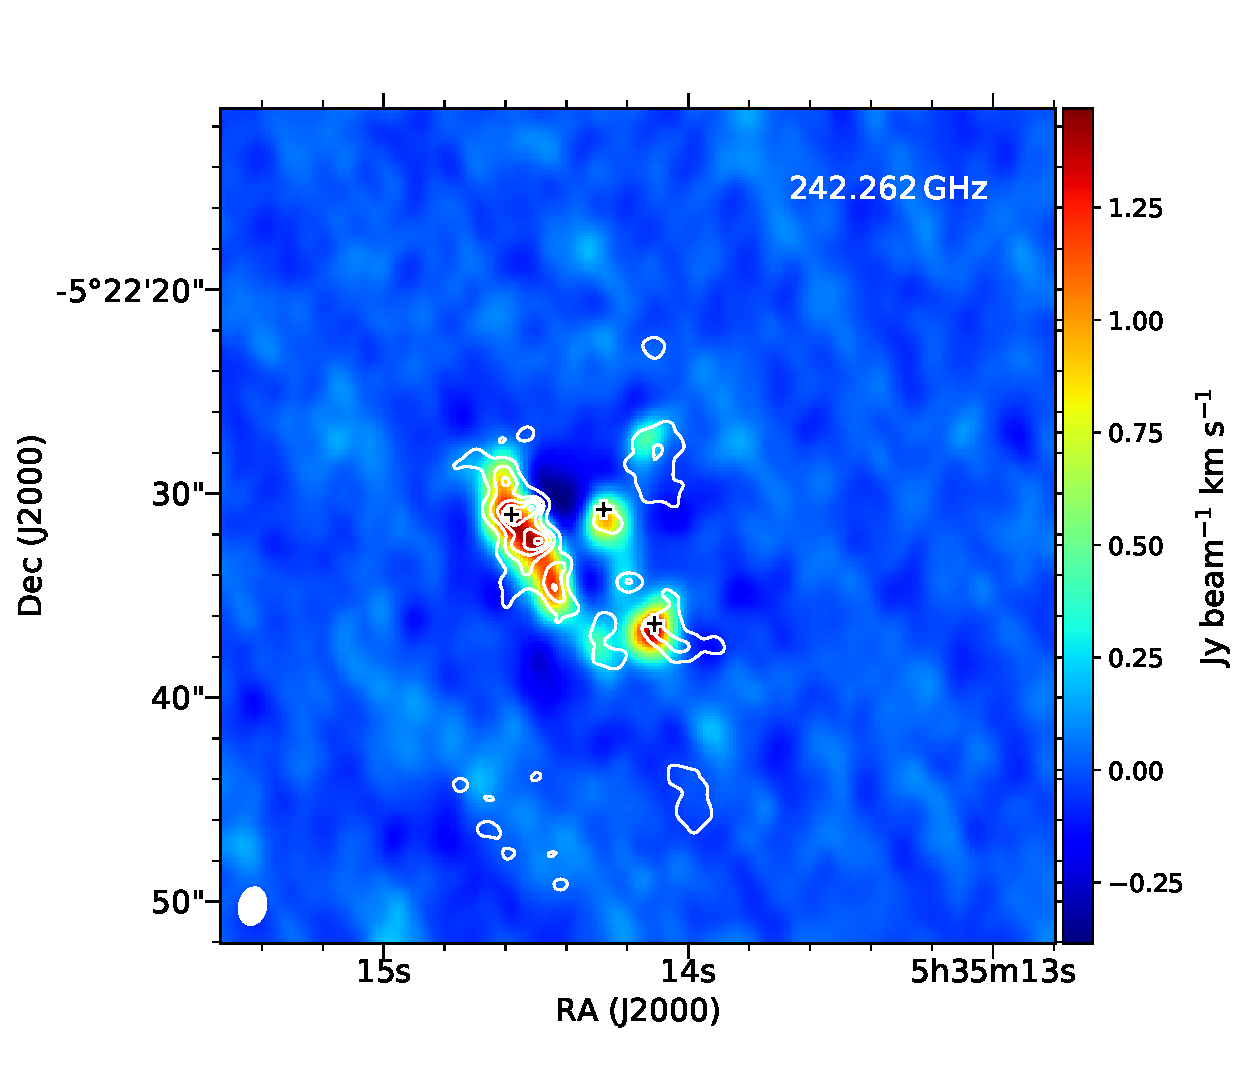
\includegraphics[width=0.98\textwidth]{OrionKL/mom0/242.262SV_mom0_3-7.eps}
%\\(g) 左の図の説明
\end{center}
\end{minipage}
\begin{minipage}{0.48\textwidth}
\begin{center}
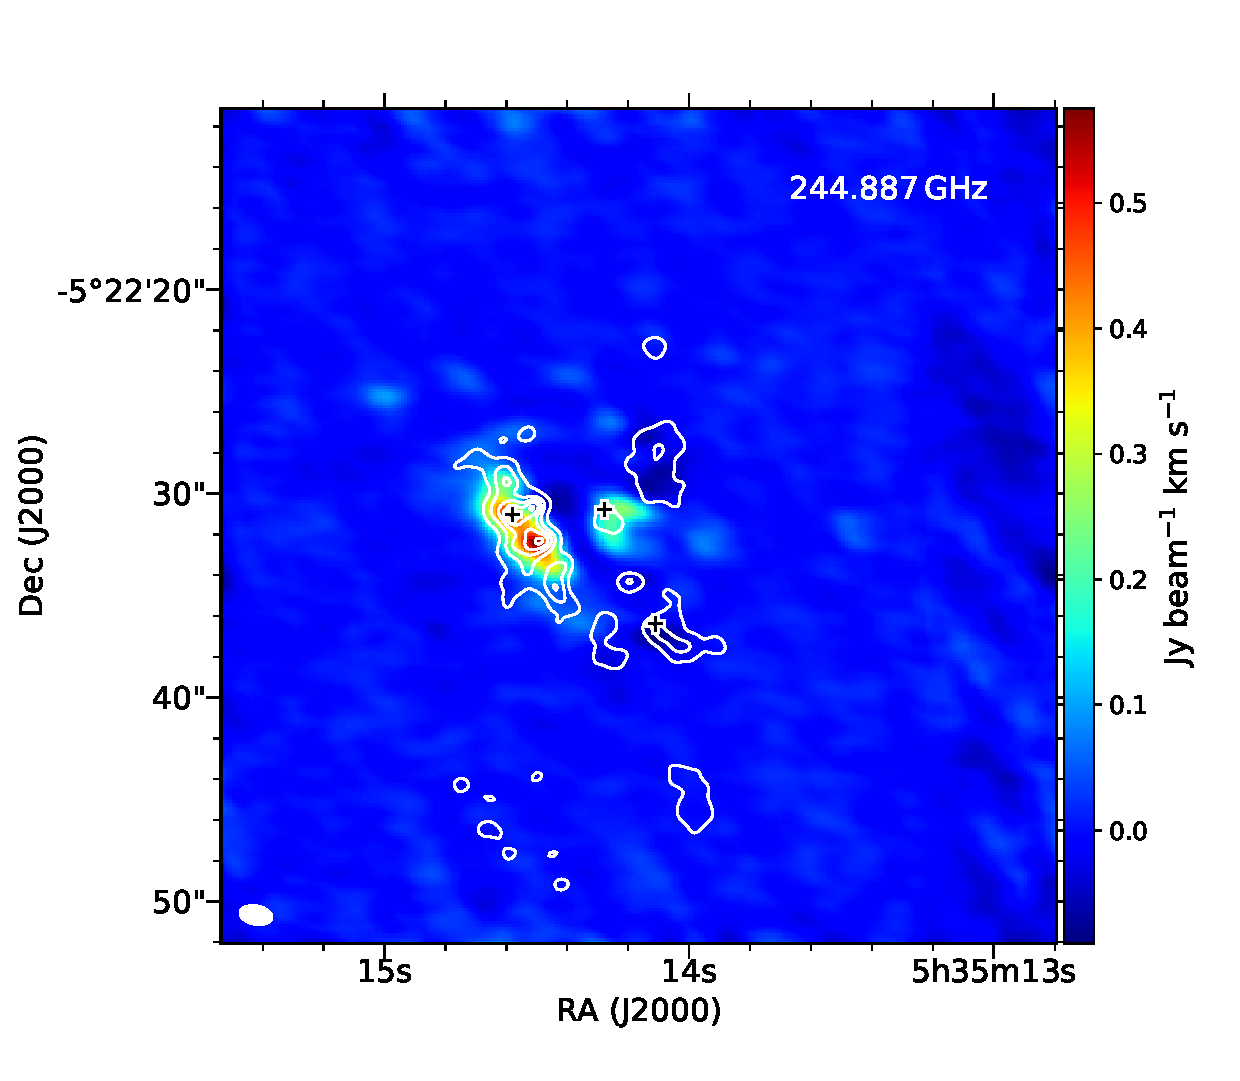
\includegraphics[width=0.98\textwidth]{OrionKL/mom0/244.887mom0_3-7.eps}
%\\(h) 右の図の説明
\end{center}
\end{minipage}
\end{center}
\end{minipage}

\caption{(Continued)}
\end{center}
\end{figure}
%%%%% 積分強度図ここまで %%%%%

%%%%%% チャネルマップここから
\begin{figure}[htbp]
  \centering
  \includegraphics[width=0.98\textwidth]{OrionKL/chmap/217.758.eps}
  \caption{217.758 GHz}
  \label{ch_0}
\end{figure}

\begin{figure}[htbp]
  \centering
  \includegraphics[width=0.98\textwidth]{OrionKL/chmap/245.202.eps}
  \caption{245.202 GHz}
  \label{ch_1}
\end{figure}

\begin{figure}[htbp]
  \centering
  \includegraphics[width=0.98\textwidth]{OrionKL/chmap/235.735.eps}
  \caption{235.735 GHz}
  \label{ch_2}
\end{figure}

\begin{figure}[htbp]
  \centering
  \includegraphics[width=0.98\textwidth]{OrionKL/chmap/242.262.eps}
  \caption{242.262 GHz}
  \label{ch_3}
\end{figure}

\begin{figure}[htbp]
  \centering
  \includegraphics[width=0.98\textwidth]{OrionKL/chmap/215.67.eps}
  \caption{215.670 GHz}
  \label{ch_4}
\end{figure}

\begin{figure}[htbp]
  \centering
  \includegraphics[width=0.98\textwidth]{OrionKL/chmap/244.887.eps}
  \caption{244.887 GHz}
  \label{ch_5}
\end{figure}

\begin{figure}[htbp]
  \centering
  \includegraphics[width=0.98\textwidth]{OrionKL/chmap/221.755.eps}
  \caption{221.755 GHz}
  \label{ch_6}
\end{figure}

\begin{figure}[htbp]
  \centering
  \includegraphics[width=0.98\textwidth]{OrionKL/chmap/229.908.eps}
  \caption{229.908 GHz}
  \label{ch_7}
\end{figure}

\subsection{Spectrum}
%%%%% スペクトル挿入 %%%%%
\begin{figure}[htbp] 
\begin{center}
\begin{minipage}{0.98\textwidth} 
\begin{center}
%%%% ここから
\begin{minipage}{0.48\textwidth}
\begin{center}
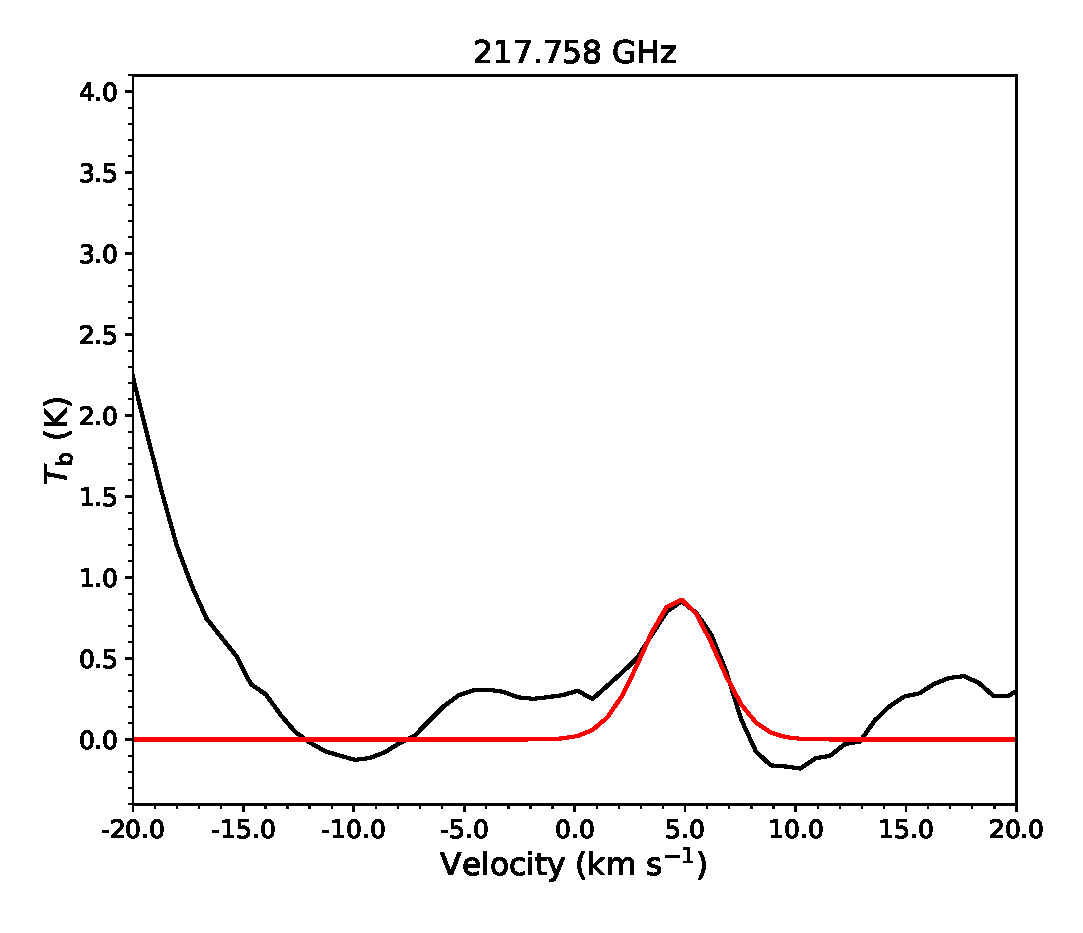
\includegraphics[width=0.98\textwidth]{OrionKL/spectrum/HC/217.758328w_fit.eps}
%\\(a) 左の図の説明
\end{center}
\end{minipage}
\begin{minipage}{0.48\textwidth}
\begin{center}
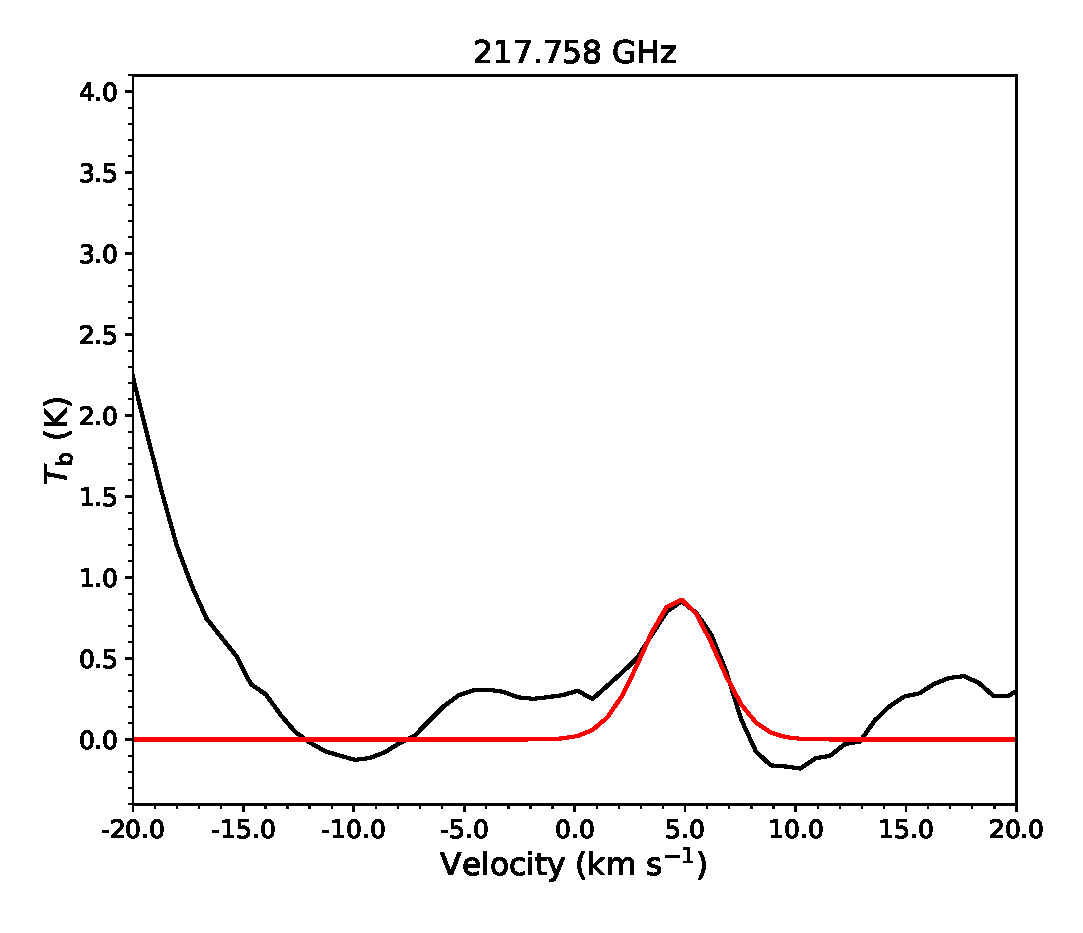
\includegraphics[width=0.98\textwidth]{OrionKL/spectrum/HC/217.758328w_fit.eps}
\\ \#(b) 245.202 GHzの図に後で差し替え
\end{center}
\end{minipage}
\end{center}
\end{minipage}
%%%% ここまで一組

\begin{minipage}{0.98\textwidth} 
\begin{center}
\begin{minipage}{0.48\textwidth}
\begin{center}
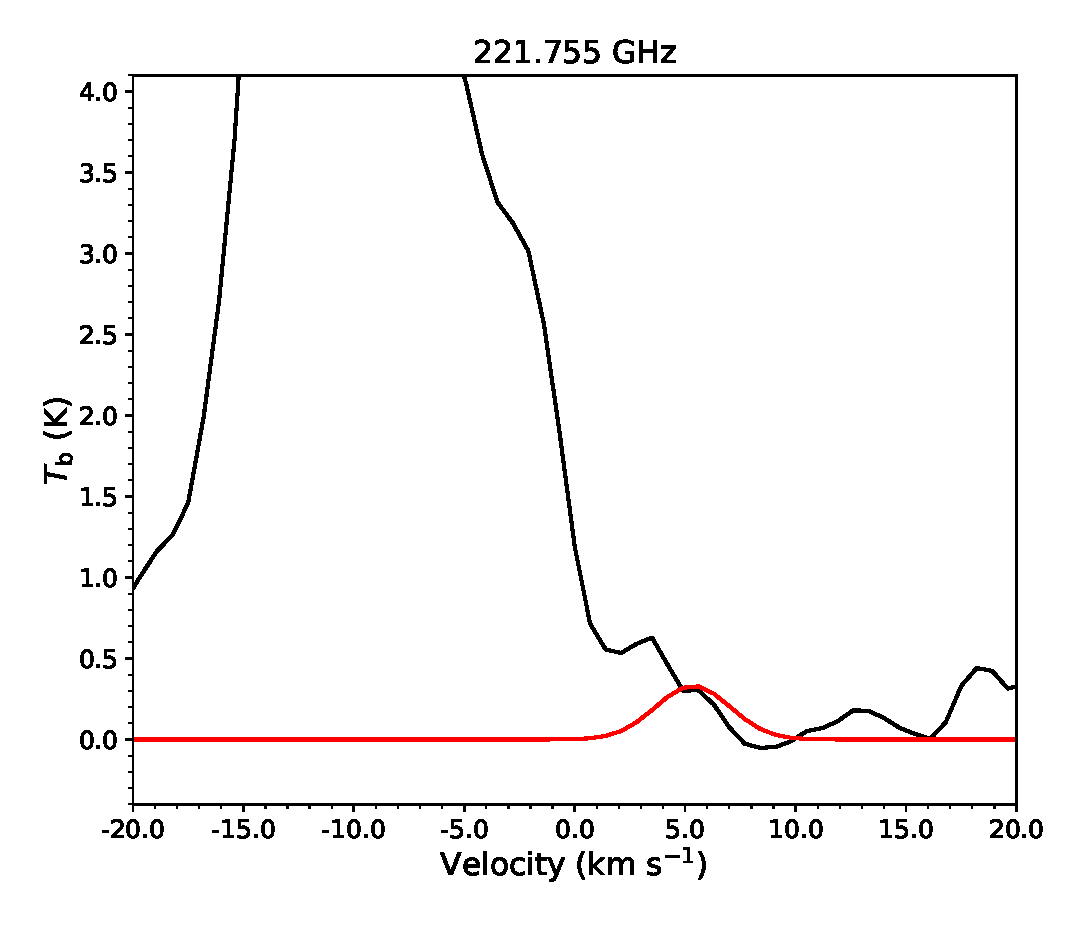
\includegraphics[width=0.98\textwidth]{OrionKL/spectrum/HC/221.755055w_fit.eps}
%\\(c) 左の図の説明
\end{center}
\end{minipage}
\begin{minipage}{0.48\textwidth}
\begin{center}
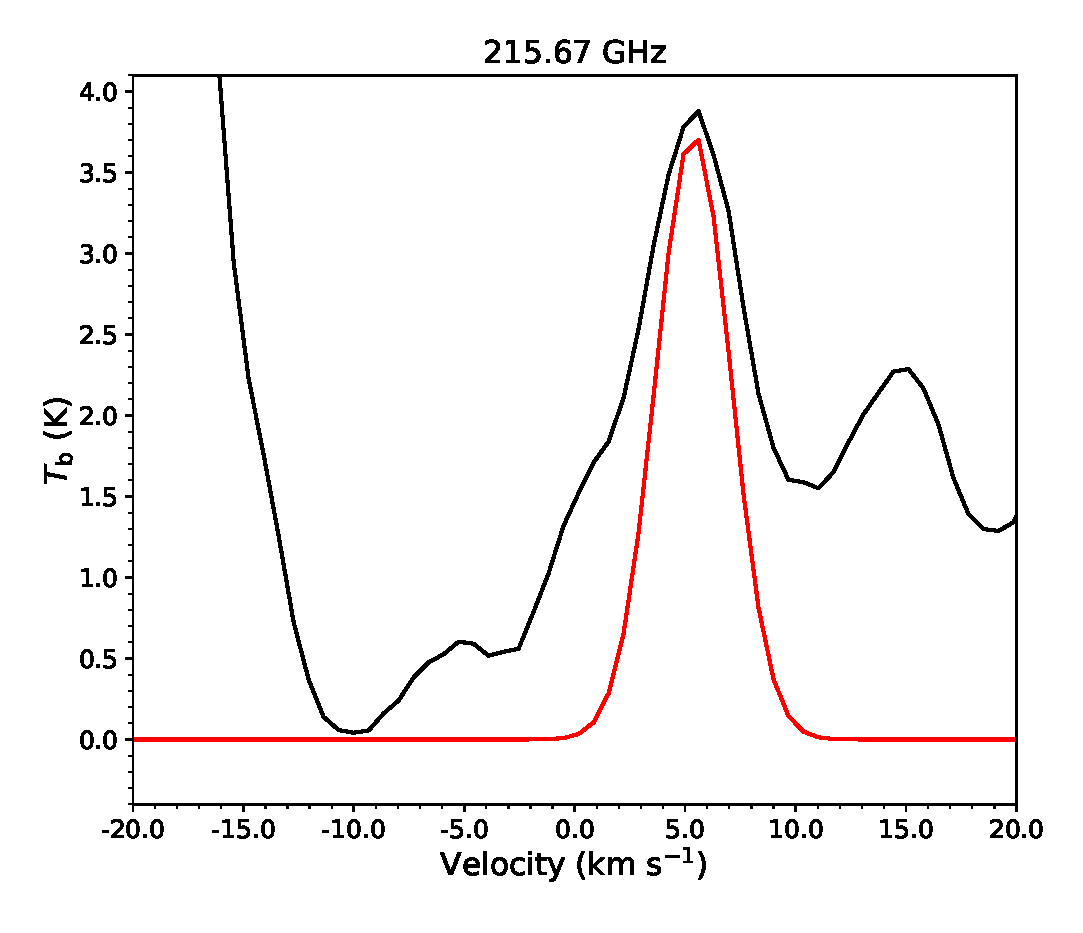
\includegraphics[width=0.98\textwidth]{OrionKL/spectrum/HC/215.6696452w_fit.eps}
%\\(d) 右の図の説明
\end{center}
\end{minipage}
\end{center}
\end{minipage}

\caption{Spectrum }
\end{center}
\end{figure}

\begin{figure}[htbp] 
\begin{center}
\begin{minipage}{0.98\textwidth} 
\begin{center}
%%%% ここから
\begin{minipage}{0.48\textwidth}
\begin{center}
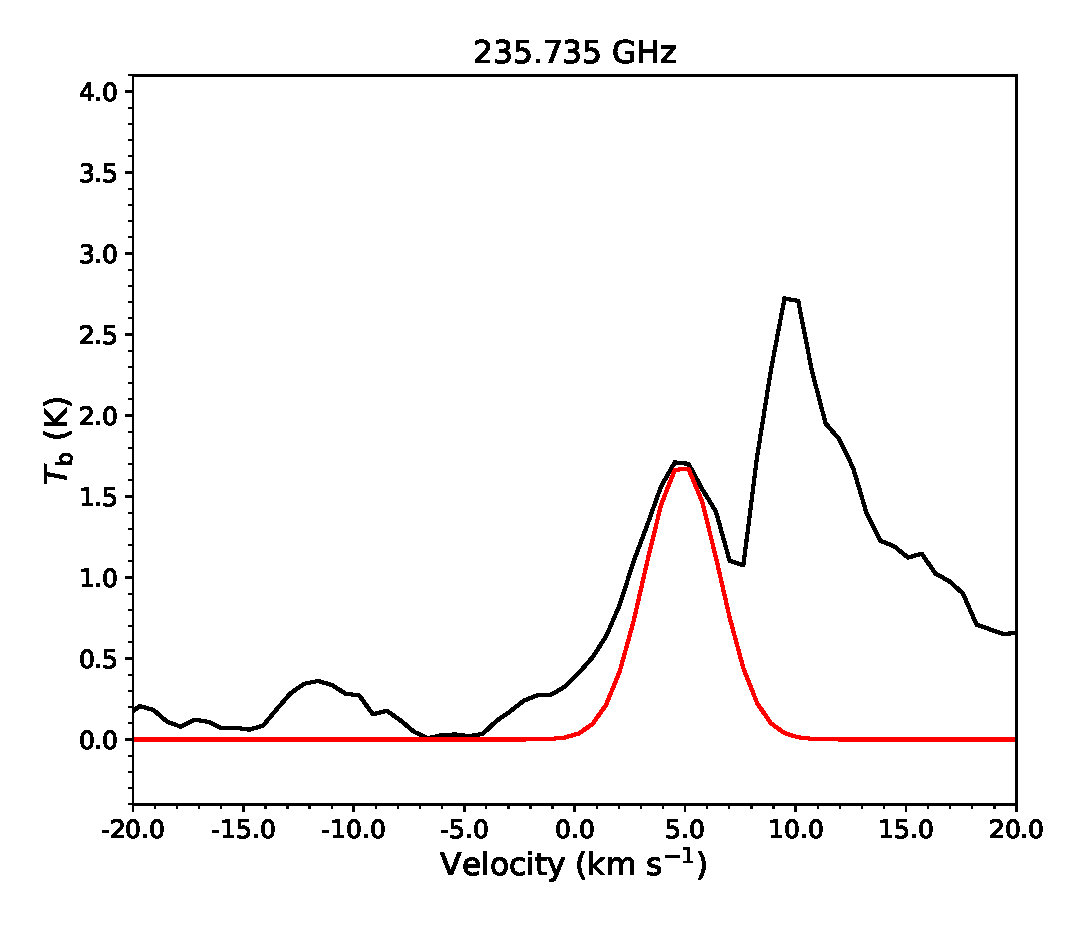
\includegraphics[width=0.98\textwidth]{OrionKL/spectrum/HC/235.735037w_fit.eps}
%\\(e) 左の図の説明
\end{center}
\end{minipage}
\begin{minipage}{0.48\textwidth}
\begin{center}
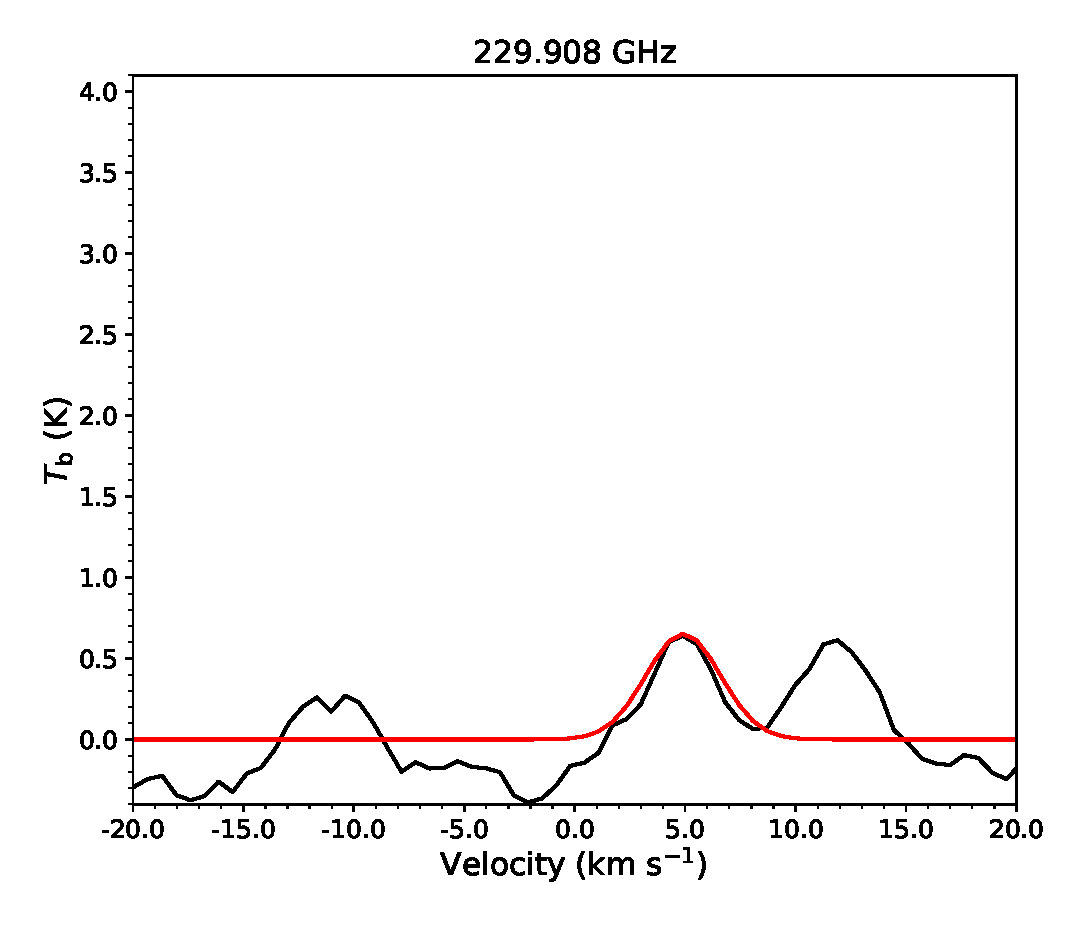
\includegraphics[width=0.98\textwidth]{OrionKL/spectrum/HC/229.908118w_fit.eps}
%\\(f) 右の図の説明
\end{center}
\end{minipage}
\end{center}
\end{minipage}
%%%% ここまで一組

\begin{minipage}{0.98\textwidth} 
\begin{center}
\begin{minipage}{0.48\textwidth}
\begin{center}
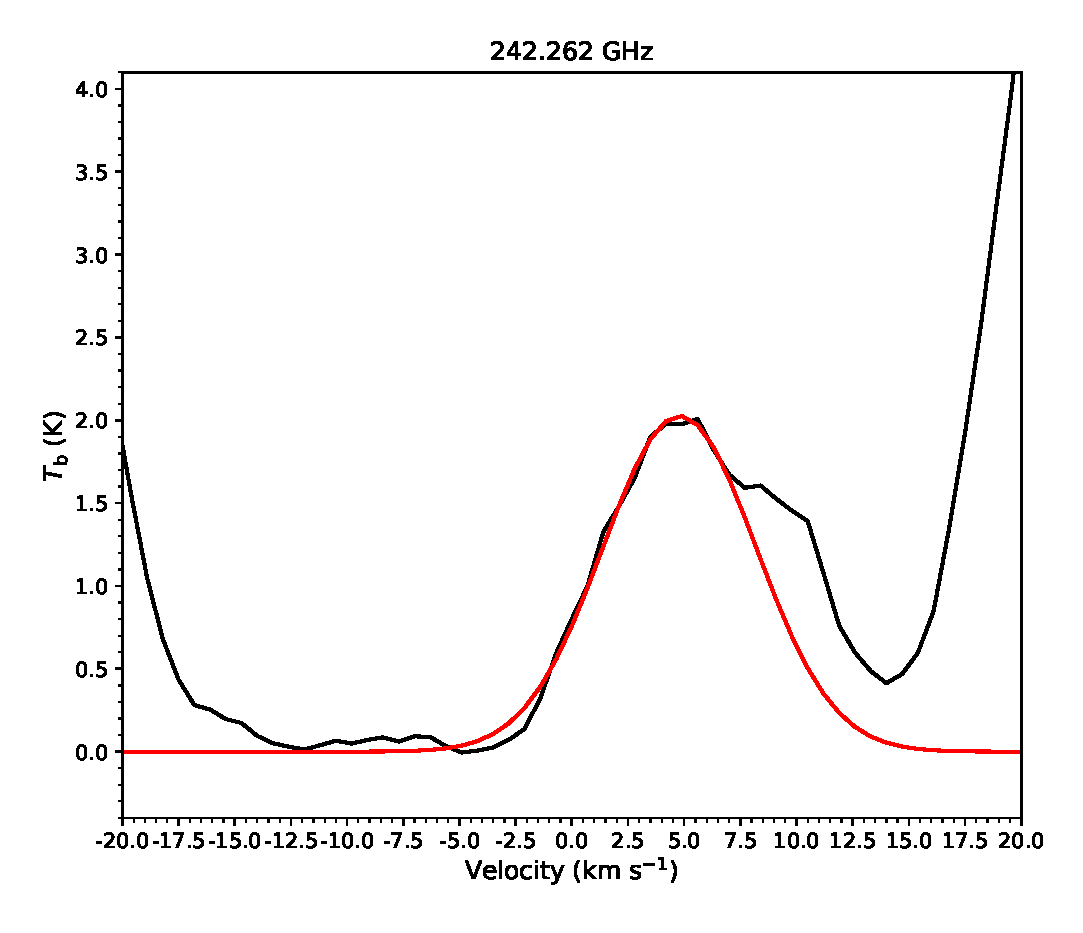
\includegraphics[width=0.98\textwidth]{OrionKL/spectrum/HC/242.2620195w_fit.eps}
%\\(g) 左の図の説明
\end{center}
\end{minipage}
\begin{minipage}{0.48\textwidth}
\begin{center}
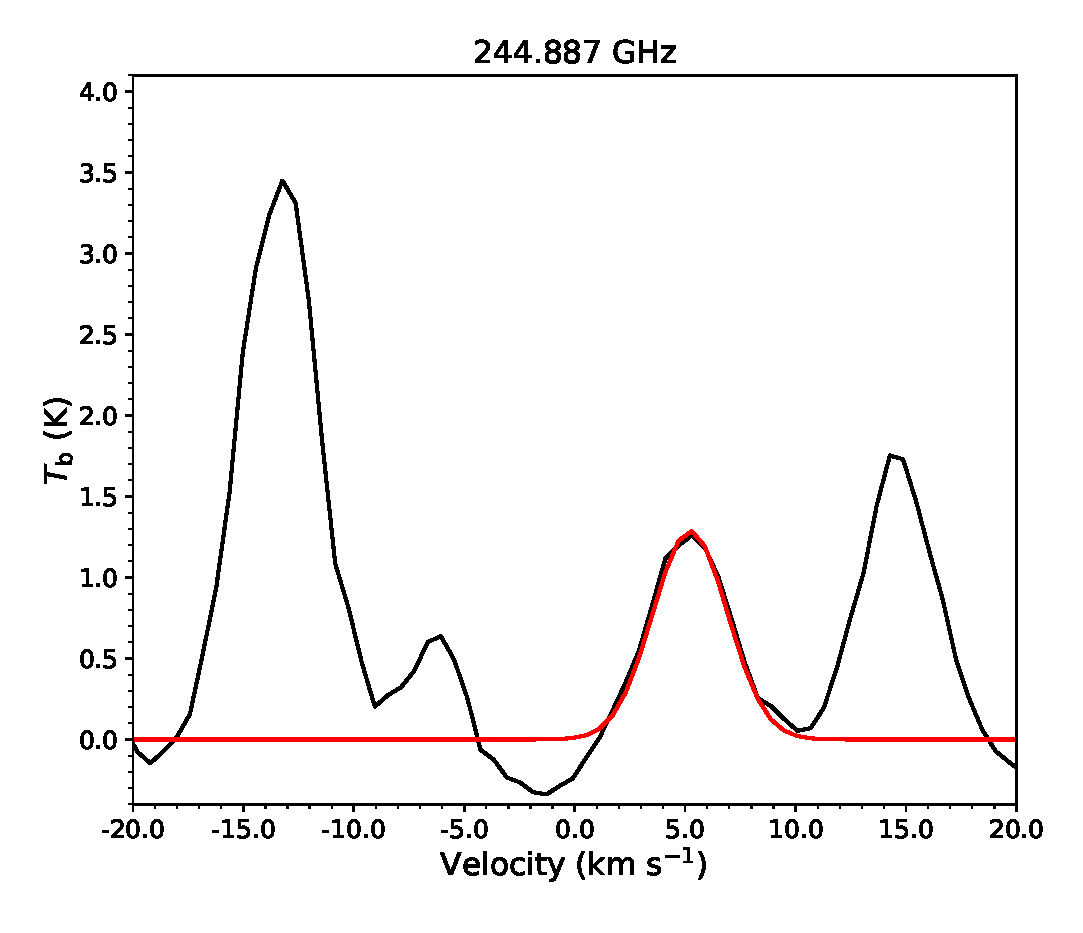
\includegraphics[width=0.98\textwidth]{OrionKL/spectrum/HC/244.8869007w_fit.eps}
%\\(h) 右の図の説明
\end{center}
\end{minipage}
\end{center}
\end{minipage}

\caption{(Continued)}
\end{center}
\end{figure}


\section{Disucssion}
\subsection{Column density and Rotation temperature}

In this subsection we will describe the methodologies in deriving fractional abundances
of COMs.

\subsection{Blending}